\documentclass[a4paper, 12pt]{article}
\usepackage[T1]{fontenc}
\usepackage{lmodern}
\usepackage{color}
\usepackage{amsfonts}
\usepackage{epstopdf}
\usepackage{matlab}
%\documentclass{book}
\usepackage{blindtext}
\usepackage{hyperref}
\usepackage[brazil]{babel}
\usepackage{amssymb}
\usepackage[utf8]{inputenc}
\usepackage{amsmath}
\usepackage{indentfirst}
\usepackage{graphicx}
\usepackage{multicol,lipsum}
\usepackage[a4paper,
top=3cm, left=3cm, bottom=3cm, right=3cm]{geometry}
\usepackage{setspace}
\usepackage{multirow}
\usepackage{float}
\usepackage[dvipsnames]{xcolor}
\usepackage[table]{xcolor}
%\usepackage{pdflscape}
\usepackage[DIV=15]{typearea}
\usepackage[nottoc]{tocbibind}
\usepackage[sort,numbers]{natbib}
%\usepackage{cite}
\usepackage{matlab}

\usepackage[utf8]{inputenc}
\usepackage[T1]{fontenc}
\usepackage{lmodern}
\usepackage{graphicx}
\usepackage{color}
\usepackage{hyperref}
\usepackage{amsmath}
\usepackage{amsfonts}
\usepackage{epstopdf}
\usepackage[table]{xcolor}
\usepackage{matlab}


\documentclass[letterpaper]{article}
% bib pack %%%%%%%%%%%%%%%%%%%%%%%%%%%%%%%%%%%%%%%%%%%%%%%%%%%%%%%%%%%%%%%%%%%%%
\usepackage[utf8]{inputenc}
\usepackage{geometry}
    \geometry{left=3cm,right=2cm,top=2cm,bottom=2cm}
%
\usepackage[spanish]{babel}
%
\usepackage[fixlanguage]{babelbib}
    \bibliographystyle{babunsrt}
%
\usepackage{url}

\begin{document}
%\maketitle

\begin{titlepage}
	\begin{center}
		

\vspace{10pt}
%\begin{figure}[H][!ht]
%\centering
%
\includegraphics{puc-rio-logo.png}

%\end{figure}
\begin{figure}[!ht]
\centering

\includegraphics{images/puc-rio-logo.png}
\end{figure}
\huge{Fundamentos de Mecatrônica}
        \vspace{70pt}
        
		\textbf{ENG1731}
		\textbf{\large{\\ }}
		
		\vspace{30pt}
		\textbf{\small{\\Lista 02}}
		\vspace{75pt}
		
	\end{center}
	
	\begin{flushleft}
		\begin{tabbing}
		Aluno(a)\qquad\qquad\=\>Paloma Fernanda Loureiro Sette - 1621595\\
			
			Professor(a)\>João Carlos Virgolino Soares\\
	\end{tabbing}
		  
	\end{flushleft}
	\begin{center}
		%\vspace{\fill}
		\vspace{215pt}
		Rio de Janeiro, 29 de Março de 2023
	\end{center}
\end{titlepage}
%%%%%%%%%%%%%%%%%%%%%%%%%%%%%%%%%%%%%%%%%%%%%%%%%%%%%%%%%%%
\newpage
\tableofcontents
\thispagestyle{empty}

\newpage
\pagenumbering{arabic}

\newpage

%\newcommand{\listequationsname}{Lista de Equações}
%\newlistof{myequations}{equ}{\listequationsname}
%\newcommand{\myequations}[1]{%
%\addcontentsline{equ}{myequations}{\protect\numberline{\theequation}#1}\par}

%\listofmyequations
\newpage


\newpage

\listoffigures
\thispagestyle{empty}

\newpage
%%%%%%%%%%%%%%%%%%%%%%%%%%%%%%%%%%%%%%%%%%%%%%%%%%%%%%%%%
%%%%%%%%%%%%%%%%%%%%%%%%%%%%%%%%%%%%%%%%%%%%%%%%%%%

\newpage

\thispagestyle{empty}

\newpage

\section{Introdução}
Este relatório refere-se ao segundo trabalho da disciplina de Fundamentos de Mecatrônica, ENG1731, de 2023.1. 

Trataremos de modelagem e simulação de um sistema mecânico representado por um pêndulo simples com duas molas, utilizando Simulink e MATLAB.

\section{Questão 01}
Para a resolução dos seguintes itens que se encontram separados por subtópicos, consideremos a figura a seguir, que mostra um sistema pêndulo simples com duas molas de constante de rigidez \textbf{k}. A massa \textbf{m} do pêndulo está concentrada na sua extremidade. Assuma que a força da mola exercida no pêndulo é nula quando ele está na vertical. Assuma também que o atrito é desprezível e o
ângulo de oscilação é pequeno. O pêndulo possui comprimento total \textbf{L}, e a distância do topo do
pêndulo até a linha das molas é a. A velocidade inicial do pêndulo é nula.

\begin{figure}[H]
\centering
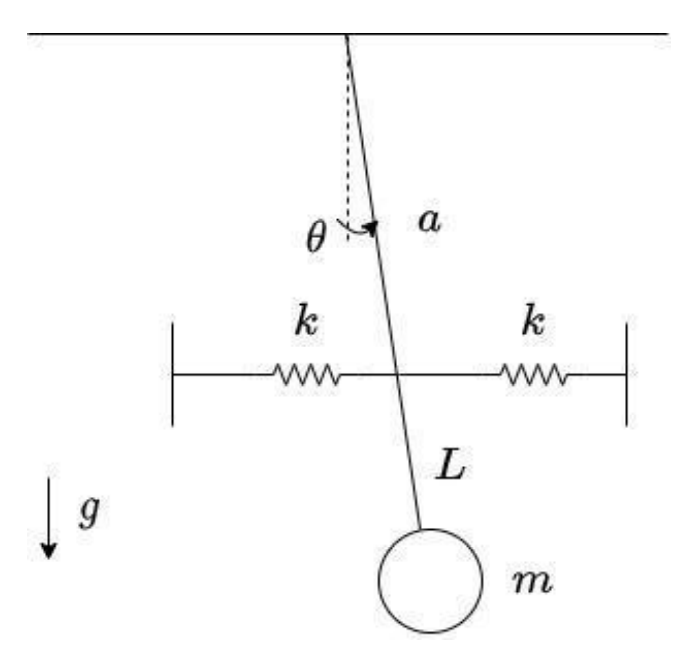
\includegraphics[scale = 0.8]{images/sistema_pendulo.PNG}
\label{filtro1}
\caption{Sistema - questão 01}
\end{figure}

\subsection{Modelo matemático do sistema}

Quando o pêndulo possui um ângulo $\theta > 0$, i.e., não está inerte,  o pêndulo é 
 "levantado" a uma distância $h = L - L cos(\theta)$. Ou seja, A energia potencial do pêndulo é:

\begin{equation}
    EP_{p} = mgh = mgL(1-cos(\theta))
\end{equation}

O nível zero se dá com o com o pêndulo na vertical. Quando o pêndulo está submetido a um ângulo não-nulo, uma das molas é comprimida por um valor $a*\theta$, enquanto a outra é esticada pela mesmo valor.
Então, a energia potencial da mola é:

\begin{equation}
    EP_{m} = \frac{1}{2} k (a*\theta)^2 * 2 = k*a^2\theta ^2
\end{equation}

Então, a energia potencial total do sistema é:

\begin{equation}
    V = mgL(1 - cos(\theta)) + k*a^2\theta ^ 2
\end{equation}

A energia cinética está associada apenas à massa $m$. A velocidade $v = L\theta$ e a energia cinética é

\begin{equation}
    T = \frac{1}{2} m L^2 \theta ^2
\end{equation}

Então, a energia total do sistema é

\begin{equation}
    E = \frac{1}{2} m L ^2 \dot \theta ^2 + mg L (1-cos(\theta)) +  K*a^2 \theta ^2
\end{equation}

Uma vez que a energia total do sistema é conservada, teremos:

\begin{equation}
    \frac{dE}{dt} = mL^2 \dot \theta \ddot \theta + mgL sin(\theta) \dot \theta + 2 k a^2 \dot \theta \theta = 0
\end{equation}

Ou, da mesma forma,

\begin{equation}\label{model_mat}
    \ddot \theta + \frac{g}{L} sin (\theta) + \frac{2 k a^2}{mL^2} \theta = 0 
\end{equation}

Logo, o modelo matemático do sistema pode ser representado pela equação \ref{model_mat}




\subsection{Resposta Analítica}
Devemos encontrar a  \textbf{resposta analítica} do sistema linearizado em torno do ponto de equilíbrio estável.
Neste caso, devemos linearizar o sistema, i.e., devemos fazer a linearização em torno de $\theta \approx 0$, onde

\begin{equation*}
    cos(\theta) \approx 1
\end{equation*}


\begin{equation*}
    sin(\theta) \approx \theta
\end{equation*}

Logo, 

\begin{equation}
    \ddot \theta + \frac{g}{L} \theta + \frac{2 k a^2}{mL^2} \theta = 0 
\end{equation}

Então, assumimos que

\begin{equation*}
    \theta(t) = {\mathrm{e}}^{\lambda t}
\end{equation*}

\begin{equation*}
    \dot \theta(t) = \lambda {\mathrm{e}}^{\lambda t}
\end{equation*}

\begin{equation*}
    \ddot \theta(t) = \lambda ^2 {\mathrm{e}}^{\lambda t}
\end{equation*}

Substituindo:
\begin{equation}
    \lambda ^2 {\mathrm{e}}^{\lambda t} + \frac{g}{L} {\mathrm{e}}^{\lambda t} + \frac{2 k a^2}{mL^2} {\mathrm{e}}^{\lambda t} = 0 
\end{equation}

\begin{equation}
   {\mathrm{e}}^{\lambda t} (\lambda ^2  + \frac{g}{L} + \frac{2 k a^2}{mL^2}) = 0 
\end{equation}

Então, nosso polinômio característico será $\lambda ^2  + \frac{g}{L} + \frac{2 k a^2}{mL^2}$.

\begin{equation}
   \lambda ^2  + \frac{g}{L} + \frac{2 k a^2}{mL^2} = 0 \Longrightarrow \lambda = \pm j \sqrt{\frac{g}{L} + \frac{2 k a^2}{mL^2}}
\end{equation}

Com isso, constatamos que teremos raízes complexas. Ou seja, nosso sistema será submetido a uma \textbf{oscilação pura}. O que faz sentido, uma vez que o sisema é desprovido de amortecimento. 


\subsection{Resposta Dinâmica}
Com base no modelo matemático obtido no tópico anterior, devemos encontrar a resposta analítica do sistema (ângulo do pêndulo em função do tempo) utilizando o Simulink.

\begin{figure}[H]
\centering
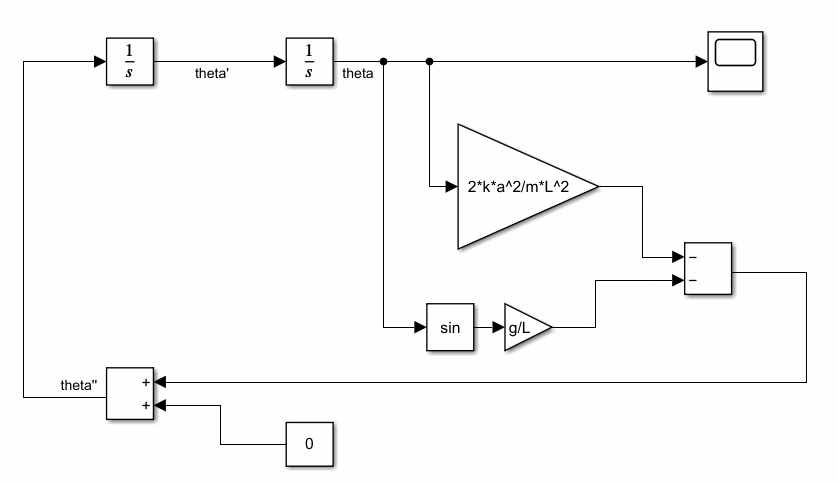
\includegraphics[scale = 0.7]{images/sistema_simulink.png}
\label{filtro1}
\caption{Sistema modelado com o Simulink}
\end{figure}


\subsection{Definição dos Parâmetros}
% This LaTeX was auto-generated from MATLAB code.
% To make changes, update the MATLAB code and export to LaTeX again.

No MATLAB, criamos um script para a definição dos parâmetros do sistema que foi compilado no Simulink.

\sloppy
\epstopdfsetup{outdir=./}
\graphicspath{ {./L01_Latex_images/} }


\begin{matlabcode}
%% LISTA 02
close all
clear
clc

%definição dos parâmetros

% Sistema pendulo simples

theta0      = 0.5;       % rad
k           = 10;        % N/m
a           = 0.6;       % m
L           = 1;         % m
m           = 1;         % kg

\end{matlabcode}


Nossa solução analítica homogênea ficará da seguinte forma

\begin{equation}
    x_h (t) = C_1 cos(\beta t ) + C_2 sin ( \beta t)
\end{equation}

De acordo com nosso polinômio característico, podemos notar que, neste caso, temos $b=0$. Faz sentido, já que estamos tratando de um sistema de oscilação pura.

\sloppy
\epstopdfsetup{outdir=./}
\graphicspath{ {./L01_Latex_images/} }


\begin{matlabcode}


A = 1;
B = 0;
C = (g/L) + (2*k*a^2)/(m*L^2);

delta = B^2 - (4*A*C)
\end{matlabcode}
\begin{matlaboutput}
delta = -68
\end{matlaboutput}
\begin{matlabcode}
lambda = (-B +sqrt(delta))/2*A
\end{matlabcode}
\begin{matlaboutput}
lambda = 0.0000 + 4.1231i
\end{matlaboutput}
\begin{matlabcode}
alpha = 0;
beta = 4.1231;

\end{matlabcode}

Temos que $x_h(0) = \theta_0 = 0.5$. Então:

\begin{equation}
    x_h(0) = C1*cos(0) + C2 * sin(0) = \frac{1}{2} \longrightarrow C1 = \frac{1}{2}
\end{equation}

Logo, nossa solução analítica homogênea será

\begin{equation}
    x_h(t) = \frac{1}{2} cos(4.1231 t )
\end{equation}

Então, podemos definir o restante dos parâmetros no MATLAB para, assim, gerarmos o gráfico da resposta analítica posteriormente.

\begin{matlabcode}
C1 = theta0;
C2 = 0;

t = 0:0.001:10;

% Equação homogênea (xh(t)):
xh = C1.*cos(beta.*t) + C2.*sin(beta.*t);

plot(t, xh);
grid on

\end{matlabcode}




\subsection{Resposta Gráfica - MATLAB e Simulink}
Devemos plotar a resposta analítica no MATLAB utilizando os mesmos parâmetros do item anterior, fazendo a comparação com o Simulink.

De acordo com os resultados obtidos anteriormente, tanto na resposta analítica quanto na resposta dinâmica, geramos os gráficos de ambas as simulações e podemos notar que as curvas resultantes são correspondentes, o que satisfaz o resultado das simulações.



\begin{figure}[H]
\centering
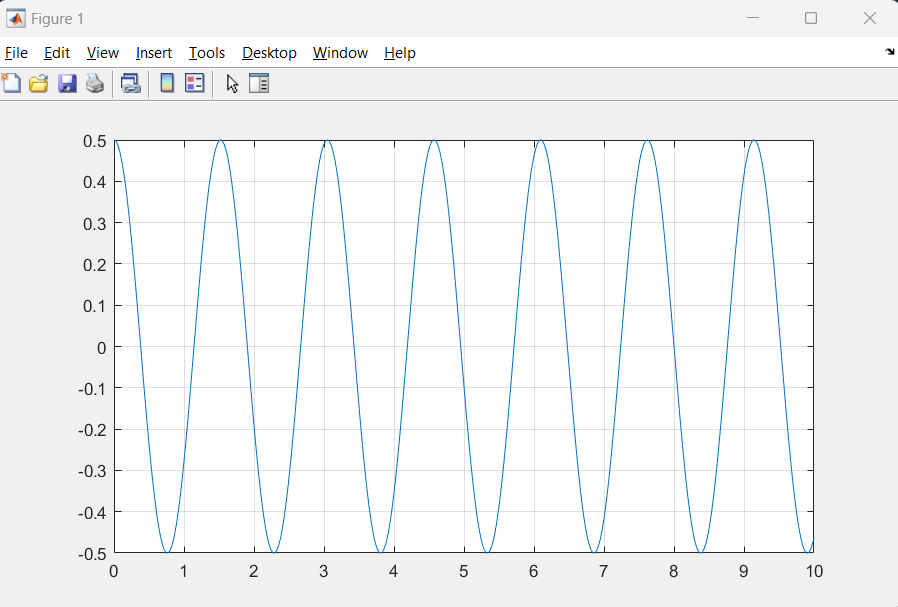
\includegraphics[scale = 0.6]{images/graph_script.png}
\label{filtro1}
\caption{Resposta gráfica gerada com o Script - Sol. analítica}
\end{figure}

\begin{figure}[H]
\centering

\includegraphics[scale = 0.6]{images/graph_simulink.png}
\label{filtro1}
\caption{Resposta gráfica gerada com o Simulink}
\end{figure}



\subsection{Pólos do Sistema}
Como sabemos, os pólos do sistema são as raízes da equação característica. Em um dos tópicos anteriores, chegamos à conclusão de que nosso polinômio característico se dá pela seguinte expressão:

\begin{equation}
    p(\lambda) = \lambda ^2  + \frac{g}{L} + \frac{2 k a^2}{mL^2}
\end{equation}

Neste caso, substituindo $g$, $L$, $k$, $m$ e $a$ pelos valores dados, teremos:

\begin{equation}
    p(\lambda) = \lambda ^2 + 17
\end{equation}

Logo, teremos que os polos do sistema serão 

\begin{equation*}
    \left(\begin{array}{c}
-\sqrt{17}\,\mathrm{i}\\
\sqrt{17}\,\mathrm{i}
\end{array}\right)
\end{equation*}


\newpage
% REFERENCIAS %%%%%%%%%%%%%%%%%%%%%%%%%%%%%%%%%%%%%%%%%%%%%%%%%%%%%%%%%%%%%%
    \nocite{*}
    \bibliography{src/bibliography}
    
\end{document}
\section{Referências Bibliográficas}



\end{document}